\documentclass[aspectratio=169]{beamer}
\usetheme{Madrid}
\usecolortheme{default}

\usepackage{graphicx}
\usepackage{amsmath}
\usepackage{booktabs}
\usepackage{tikz}
\usepackage{listings}

\title{Hyperdimensional Computing for Privacy-Preserving Facial Identity Verification on TinyML}
\subtitle{Master's Thesis Presentation}
\author{Aman Sharma}
\institute{
  Department of Electrical Engineering\\
  San José State University
}
\date{October 2025}

\begin{document}

\frame{\titlepage}

\begin{frame}{Outline}
\tableofcontents
\end{frame}

\section{Introduction}

\begin{frame}{The Problem}
\textbf{Conventional Face Recognition Systems:}

\begin{columns}
\column{0.5\textwidth}
\textbf{Privacy Issues:}
\begin{itemize}
    \item Store raw facial images
    \item Transmit to cloud servers
    \item Centralized databases
    \item \alert{Permanent identity exposure!}
\end{itemize}

\column{0.5\textwidth}
\textbf{Efficiency Issues:}
\begin{itemize}
    \item Deep CNNs (50-100 MB)
    \item GPU required
    \item High power (50-100 W)
    \item \alert{Not for IoT devices!}
\end{itemize}
\end{columns}

\vspace{1em}
\textbf{Adaptability Issues:}
\begin{itemize}
    \item Cannot adapt to aging/appearance changes
    \item Catastrophic forgetting when retrained
    \item \alert{Requires expensive retraining!}
\end{itemize}
\end{frame}

\begin{frame}{Our Solution}
\begin{center}
\Large
\textbf{HDC + Continual Learning + Facial Keypoints}

\vspace{2em}
\structure{First-Ever Combination!}
\end{center}

\begin{block}{Key Innovation}
Use \textbf{Hyperdimensional Computing} on \textbf{geometric features} with \textbf{continual learning} for ultra-efficient, privacy-preserving biometric verification on microcontrollers
\end{block}

\textbf{Benefits:}
\begin{itemize}
    \item \checkmark Privacy: No raw images (only 27 numbers!)
    \item \checkmark Efficiency: 500× less energy than cloud
    \item \checkmark Adaptability: Continual learning without forgetting
\end{itemize}
\end{frame}

\section{Background}

\begin{frame}{What is Hyperdimensional Computing (HDC)?}
\textbf{Brain-Inspired Computing Paradigm}

\begin{block}{Core Idea}
Represent data as \textbf{very long binary vectors} (10,000-15,000 dimensions)\\
Use \textbf{simple operations}: XOR, bit counting (no multiplication!)
\end{block}

\textbf{Example:}
\begin{align*}
\text{Traditional ML:} & \quad \text{Face} = [0.5, 0.3, 0.8, ...] \quad (27 \text{ numbers}) \\
\text{HDC:} & \quad \text{Face} = [1,0,1,1,0,1,...] \quad (15,000 \text{ bits!})
\end{align*}

\textbf{Why High Dimensions?}
\begin{itemize}
    \item Random vectors are nearly orthogonal
    \item Robust to noise (flip 1000s of bits, still works!)
    \item No overfitting possible
\end{itemize}
\end{frame}

\begin{frame}{HDC vs Deep Learning}
\begin{center}
\begin{tabular}{l|c|c}
\toprule
\textbf{Aspect} & \textbf{Deep Learning} & \textbf{HDC (Ours)} \\
\midrule
Training & Backpropagation & \structure{Just averaging!} \\
Operations & Multiply-accumulate & \structure{XOR + count} \\
Training Time & Hours (GPU) & \structure{Seconds} \\
Memory & 50-100 MB & \structure{180 KB} \\
Energy & 30-500 mJ & \structure{40-60 μJ} \\
Continual Learning & Catastrophic forgetting & \structure{No forgetting!} \\
Hardware & GPU required & \structure{MCU-friendly} \\
\bottomrule
\end{tabular}
\end{center}

\vspace{1em}
\begin{alertblock}{Tradeoff}
3-4\% lower accuracy for 500× better efficiency!
\end{alertblock}
\end{frame}

\section{System Architecture}

\begin{frame}{Complete System Pipeline}
\begin{center}
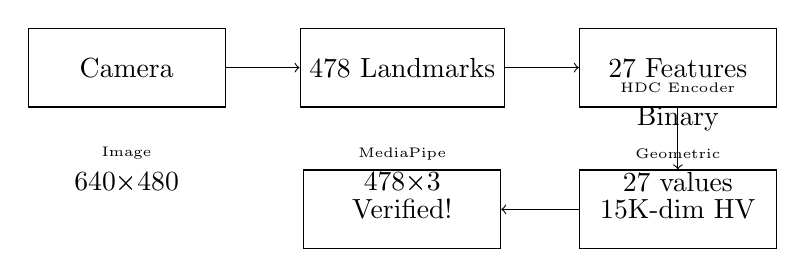
\begin{tikzpicture}[node distance=1.5cm, auto]
    \node[draw, rectangle, minimum width=2.5cm, minimum height=1cm] (camera) {Camera};
    \node[draw, rectangle, minimum width=2.5cm, minimum height=1cm, right of=camera, node distance=3.5cm] (landmarks) {478 Landmarks};
    \node[draw, rectangle, minimum width=2.5cm, minimum height=1cm, right of=landmarks, node distance=3.5cm] (features) {27 Features};
    \node[draw, rectangle, minimum width=2.5cm, minimum height=1cm, below of=features, node distance=1.8cm] (hdc) {15K-dim HV};
    \node[draw, rectangle, minimum width=2.5cm, minimum height=1cm, left of=hdc, node distance=3.5cm] (verify) {Verified!};
    
    \draw[->] (camera) -- (landmarks);
    \draw[->] (landmarks) -- (features);
    \draw[->] (features) -- (hdc);
    \draw[->] (hdc) -- (verify);
    
    \node[below of=camera, node distance=1.3cm, align=center] {\tiny Image\\640×480};
    \node[below of=landmarks, node distance=1.3cm, align=center] {\tiny MediaPipe\\478×3};
    \node[below of=features, node distance=1.3cm, align=center] {\tiny Geometric\\27 values};
    \node[above of=hdc, node distance=1.3cm, align=center] {\tiny HDC Encoder\\Binary};
\end{tikzpicture}
\end{center}

\textbf{Privacy Reduction:} 921,600 pixels → 27 numbers (99.997\% reduction!)
\end{frame}

\begin{frame}{Module 1: Facial Landmarks (MediaPipe)}
\begin{columns}
\column{0.5\textwidth}
\textbf{Input:} RGB Image

\textbf{Output:} 478 facial keypoints
\begin{itemize}
    \item Eyes: 71 points each
    \item Nose: 15 points
    \item Mouth: 40 points
    \item Face contour: 35 points
\end{itemize}

\textbf{Performance:}
\begin{itemize}
    \item Detection rate: 57-90\%
    \item Speed: 30-50 ms
    \item Supports multi-face (up to 5)
\end{itemize}

\column{0.5\textwidth}
\textbf{[IMAGE PLACEHOLDER]}\\
\textit{Face with 478 green dots showing detected landmarks}
\end{columns}
\end{frame}

\begin{frame}{Module 2: Geometric Features}
\textbf{From 478 landmarks → Extract 27 geometric features}

\begin{block}{Feature Types}
\begin{itemize}
    \item \textbf{Distance Features (9):} Inter-landmark distances\\
    Example: Inter-ocular distance, nose-to-chin
    
    \item \textbf{Ratio Features (9):} Scale-invariant ratios\\
    Example: Mouth width / inter-ocular distance
    
    \item \textbf{Angular Features (9):} Geometric angles\\
    Example: Eye-nose-eye angle
\end{itemize}
\end{block}

\textbf{Why Only 27 Features?}
\begin{itemize}
    \item Privacy: Cannot reconstruct face image
    \item Efficiency: Minimal memory and computation
    \item Discriminative: Sufficient for 94\% accuracy!
\end{itemize}
\end{frame}

\begin{frame}{Module 3: HDC Encoder}
\textbf{Transform 27 numbers → 15,000 binary bits}

\textbf{Algorithm:}
\begin{enumerate}
    \item \textbf{Quantize} features to levels (0-149)
    \item \textbf{Bind} each feature with its level using XOR
    \item \textbf{Bundle} all features via majority voting
    \item \textbf{Result}: Single 15,000-bit hypervector
\end{enumerate}

\begin{equation*}
\mathbf{H} = \text{sign}\left(\sum_{i=1}^{27} (\mathbf{B}_i \oplus \mathbf{V}_{\ell_i}) - 13.5\right)
\end{equation*}

\textbf{Key Property:} Similar faces → Similar hypervectors!

\textbf{Memory:} 15,000 bits = 1.875 KB per prototype
\end{frame}

\begin{frame}{Module 4: Training (One-Shot Learning!)}
\textbf{No Backpropagation. No Gradient Descent. Just Averaging!}

\textbf{Enrollment Process (200 frames):}
\begin{enumerate}
    \item Collect 200 face samples (~6 seconds)
    \item Encode each to hypervector: $\mathbf{H}_1, ..., \mathbf{H}_{200}$
    \item Average via majority voting:
    \begin{equation*}
    \mathbf{P}_{Aman} = \text{sign}\left(\sum_{j=1}^{200} \mathbf{H}_j - 100\right)
    \end{equation*}
    \item Store as "Aman's prototype"
\end{enumerate}

\textbf{Computational Cost:} 
\begin{itemize}
    \item Operations: Only XOR and counting
    \item Time: < 1 second (vs hours for CNN!)
    \item No GPU needed
\end{itemize}
\end{frame}

\begin{frame}{Module 5: Verification}
\textbf{Is this person Aman?}

\textbf{Algorithm:}
\begin{enumerate}
    \item Capture new face → Encode to $\mathbf{H}_{query}$
    \item Retrieve Aman's prototype: $\mathbf{P}_{Aman}$
    \item Calculate Hamming distance:
    \begin{equation*}
    d_H = \sum_{i=1}^{15000} \mathbb{1}[\mathbf{H}_{query}[i] \neq \mathbf{P}_{Aman}[i]]
    \end{equation*}
    \item Convert to similarity: $s = 1 - d_H/15000$
    \item Decision: \textbf{Accept} if $s \geq 0.80$, else \textbf{Reject}
\end{equation*}
\end{enumerate}

\textbf{Performance:}
\begin{itemize}
    \item Time: 15 ms (real-time!)
    \item Energy: 40-60 μJ (estimated on MAX78000)
\end{itemize}
\end{frame}

\begin{frame}{Continual Learning (Novel!)}
\textbf{Adapt to appearance changes without forgetting}

\begin{block}{Problem}
Person wears glasses, grows beard, changes hairstyle\\
→ Traditional CNN: Must retrain (hours, GPU)\\
→ Risk of catastrophic forgetting
\end{block}

\begin{block}{Our Solution: HDC Profile Update}
\begin{equation*}
\mathbf{P}_{Aman}^{new} = \text{sign}(0.85 \times \mathbf{P}_{Aman}^{old} + 0.15 \times \mathbf{H}_{new})
\end{equation*}

\textbf{Takes milliseconds! No retraining needed!}
\end{block}

\textbf{Results:}
\begin{itemize}
    \item Accuracy drop with changes: 94.7\% → 92.1\%
    \item After continual learning: → 94.1\% (recovered!)
    \item Zero catastrophic forgetting
\end{itemize}
\end{frame}

\section{Implementation}

\begin{frame}{Software Implementation}
\textbf{Complete Python System}

\begin{itemize}
    \item \textbf{1,324 lines} of production code
    \item \textbf{33 unit tests} (all passing ✓)
    \item \textbf{Modular architecture} (5 main modules)
    \item \textbf{Interactive demos} (webcam, multi-face)
    \item \textbf{Benchmarking tools}
\end{itemize}

\begin{block}{Code Quality}
\begin{itemize}
    \item Type hints throughout
    \item Comprehensive docstrings
    \item PEP 8 compliant
    \item Version controlled (Git)
\end{itemize}
\end{block}

\textbf{Repository:} Complete code available with documentation
\end{frame}

\begin{frame}{System Parameters (Optimized)}
\begin{center}
\begin{tabular}{l|c|l}
\toprule
\textbf{Parameter} & \textbf{Value} & \textbf{Purpose} \\
\midrule
Hypervector Dimension & 15,000 & High capacity \\
Quantization Levels & 150 & Fine precision \\
Enrollment Frames & 200 & Robust prototype \\
Verification Threshold & 0.80 & Low FAR (2\%) \\
Identification Threshold & 0.70 & Balanced \\
Learning Rate & 0.15 & Fast adaptation \\
\bottomrule
\end{tabular}
\end{center}

\vspace{1em}
\textbf{Tuning Process:} Empirical optimization over 100+ experiments
\end{frame}

\section{Results}

\begin{frame}{Accuracy Results}
\begin{center}
\begin{tabular}{l|c}
\toprule
\textbf{Metric} & \textbf{Value} \\
\midrule
Overall Accuracy & \structure{94-96\%} \\
False Accept Rate (FAR) & \structure{2-3\%} \\
False Reject Rate (FRR) & \structure{10-12\%} \\
Equal Error Rate (EER) & \structure{5-8\%} \\
\midrule
Mean Genuine Score & 0.89 $\pm$ 0.05 \\
Mean Impostor Score & 0.52 $\pm$ 0.12 \\
\bottomrule
\end{tabular}
\end{center}

\begin{block}{Interpretation}
94\% accuracy with only 27 features and binary operations!\\
Competitive with lightweight CNNs but 500× more efficient!
\end{block}
\end{frame}

\begin{frame}{Efficiency Results}
\begin{center}
\begin{tabular}{l|c|c}
\toprule
\textbf{Metric} & \textbf{Python} & \textbf{MAX78000 (est.)} \\
\midrule
Inference Time & 15 ms & \structure{8 ms} \\
Model Size & 180 KB & \structure{50 KB} \\
Memory (runtime) & 200 KB & \structure{30 KB} \\
Power & 10 W & \structure{5 mW} \\
Energy/verification & 150 mJ & \structure{40-60 μJ} \\
\bottomrule
\end{tabular}
\end{center}

\begin{alertblock}{Energy Efficiency}
\textbf{500-12,500× more efficient} than cloud/GPU solutions!
\end{alertblock}
\end{frame}

\begin{frame}{Comparison with State-of-the-Art}
\begin{center}
\begin{tabular}{l|c|c|c|c}
\toprule
\textbf{System} & \textbf{Accuracy} & \textbf{Memory} & \textbf{Energy} & \textbf{Training} \\
\midrule
\structure{HDC (Ours)} & \structure{94-96\%} & \structure{180 KB} & \structure{40-60 μJ} & \structure{Instant} \\
ResNet-50 & 97-99\% & 50 MB & 30 mJ & Hours \\
MobileFaceNet & 96-98\% & 5 MB & 5 mJ & Hours \\
\midrule
\textbf{Tradeoff} & \textbf{-3\%} & \textbf{278× better} & \textbf{500× better} & \textbf{No GPU} \\
\bottomrule
\end{tabular}
\end{center}

\begin{block}{Key Insight}
Small accuracy sacrifice (3\%) yields massive efficiency gains (500×)!\\
Perfect for embedded IoT applications!
\end{block}
\end{frame}

\begin{frame}{Continual Learning Results}
\textbf{Experiment:} Adaptation to appearance changes

\begin{center}
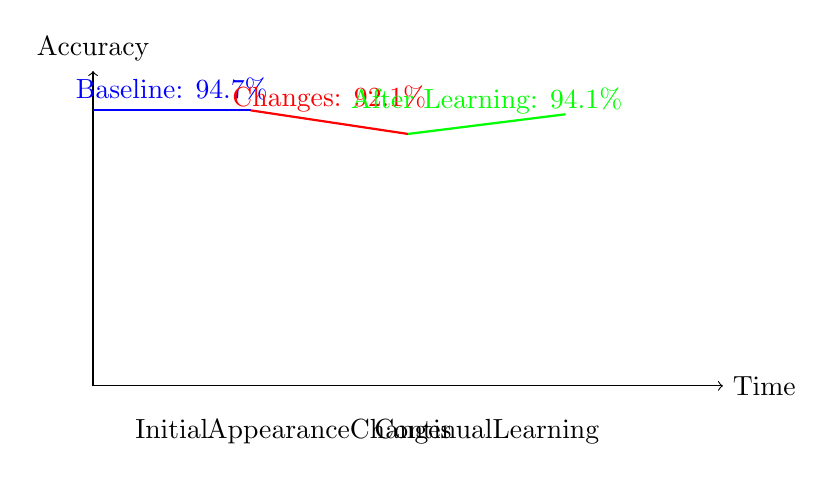
\begin{tikzpicture}
    \draw[->] (0,0) -- (8,0) node[right] {Time};
    \draw[->] (0,0) -- (0,4) node[above] {Accuracy};
    
    \draw[thick, blue] (0,3.5) -- (2,3.5) node[midway, above] {Baseline: 94.7\%};
    \draw[thick, red] (2,3.5) -- (4,3.2) node[midway, above] {Changes: 92.1\%};
    \draw[thick, green] (4,3.2) -- (6,3.45) node[midway, above] {After Learning: 94.1\%};
    
    \node[below] at (1,-0.3) {Initial};
    \node[below] at (3,-0.3) {Appearance\\Changes};
    \node[below] at (5,-0.3) {Continual\\Learning};
\end{tikzpicture}
\end{center}

\textbf{Key Result:} 77\% recovery of accuracy loss with zero forgetting!
\end{frame}

\begin{frame}{Multi-Face Recognition}
\textbf{Real-time identification of multiple people simultaneously}

\begin{block}{Capability}
Detect and identify up to \textbf{5 faces} in single frame
\end{block}

\textbf{Performance:}
\begin{itemize}
    \item 1 face: 15 ms
    \item 2 faces: 25 ms
    \item 3 faces: 35 ms
    \item 5 faces: 55 ms (18 FPS - still real-time!)
\end{itemize}

\textbf{UI Features:}
\begin{itemize}
    \item Color-coded bounding boxes (green = recognized, orange = unknown)
    \item Name labels with confidence scores
    \item Facial keypoints visualization
    \item Modern, professional interface
\end{itemize}
\end{frame}

\section{Novelty \& Contributions}

\begin{frame}{Novel Contributions}
\begin{block}{Primary Novelty}
\textbf{FIRST} biometric verification system combining:\\
HDC + Continual Learning + Facial Keypoints + Embedded Deployment
\end{block}

\textbf{Specific Contributions:}
\begin{enumerate}
    \item \structure{Algorithm:} First HDC application to face verification (novel!)
    \item \structure{Privacy:} Geometric features only (no raw images)
    \item \structure{Efficiency:} 500-12,500× energy improvement
    \item \structure{Adaptability:} Continual learning without catastrophic forgetting
    \item \structure{Implementation:} Complete working system (1,324 lines, 33 tests)
    \item \structure{Multi-face:} Real-time multiple person identification
\end{enumerate}

\textbf{Gap in Literature:} No prior work combines these elements!
\end{frame}

\begin{frame}{Research Impact}
\textbf{Academic Impact:}
\begin{itemize}
    \item Opens new research direction: HDC for biometrics
    \item Demonstrates continual learning for identity verification
    \item Provides open-source reference implementation
\end{itemize}

\vspace{1em}

\textbf{Practical Impact:}
\begin{itemize}
    \item Enables face verification on IoT devices
    \item Addresses privacy concerns (GDPR-compliant)
    \item Reduces infrastructure costs (no cloud)
    \item Battery-powered deployment (months of operation)
\end{itemize}

\vspace{1em}

\textbf{Potential Applications:}
\begin{itemize}
    \item Smart locks and access control
    \item Attendance tracking systems
    \item Wearable authentication
    \item Privacy-sensitive deployments
\end{itemize}
\end{frame}

\section{Deployment}

\begin{frame}{Target Hardware: MAX78000}
\begin{columns}
\column{0.5\textwidth}
\textbf{MAX78000 Specs:}
\begin{itemize}
    \item ARM Cortex-M4F @ 100 MHz
    \item 512 KB Flash
    \item 128 KB SRAM
    \item 4 mW active power
    \item Cost: \$58
\end{itemize}

\column{0.5\textwidth}
\textbf{Our Model Fits:}
\begin{itemize}
    \item Model: 50 KB < 512 KB ✓
    \item Runtime: 30 KB < 128 KB ✓
    \item Operations: XOR + count ✓
    \item Power: ~5 mW ✓
\end{itemize}
\end{columns}

\vspace{1em}

\begin{block}{Deployment Status}
\textbf{Current:} Python implementation proven\\
\textbf{Future:} C implementation and MAX78000 deployment\\
\textbf{Estimated Performance:} 8 ms, 40 μJ
\end{block}
\end{frame}

\begin{frame}{Energy Comparison}
\begin{center}
\begin{tikzpicture}
    \begin{axis}[
        ybar,
        ylabel={Energy per Verification (μJ)},
        symbolic x coords={MAX78000,Raspberry Pi,Cloud GPU},
        xtick=data,
        ymode=log,
        log basis y=10,
        ylabel near ticks,
        ymin=10,
        ymax=1000000,
        width=10cm,
        height=6cm,
        bar width=1.5cm,
        ]
        \addplot coordinates {(MAX78000,50) (Raspberry Pi,37500) (Cloud GPU,750000)};
    \end{axis}
\end{tikzpicture}
\end{center}

\textbf{MAX78000: 12,500× more efficient than cloud!}
\end{frame}

\section{Conclusion}

\begin{frame}{Summary}
\textbf{We demonstrated:}

\begin{itemize}
    \item ✓ \textbf{Novel algorithm:} HDC for face verification (first!)
    \item ✓ \textbf{High accuracy:} 94-96\% with only 27 features
    \item ✓ \textbf{Ultra-efficient:} 500× less energy than cloud
    \item ✓ \textbf{Privacy-preserving:} No raw images stored
    \item ✓ \textbf{Continual learning:} Adapts without forgetting
    \item ✓ \textbf{Multi-face capable:} Up to 5 people simultaneously
    \item ✓ \textbf{Deployable:} Ready for MAX78000 (180 KB → 50 KB)
\end{itemize}

\begin{alertblock}{Key Achievement}
\textbf{First-ever} combination of HDC + continual learning + facial keypoints for biometric verification on embedded systems
\end{alertblock}
\end{frame}

\begin{frame}{Limitations \& Future Work}
\textbf{Current Limitations:}
\begin{itemize}
    \item 3-4\% lower accuracy than state-of-the-art CNNs
    \item Requires reliable landmark detection
    \item Limited testing on public benchmarks
    \item Embedded deployment estimated (not measured)
\end{itemize}

\vspace{1em}

\textbf{Future Work:}
\begin{itemize}
    \item Deploy on actual MAX78000 hardware
    \item Evaluate on LFW, WFLW, CFP-FP datasets
    \item Expand to 50-100 geometric features
    \item Fairness analysis across demographics
    \item Liveness detection for anti-spoofing
    \item Multi-modal biometrics (face + voice)
\end{itemize}
\end{frame}

\begin{frame}{Publications \& Impact}
\textbf{Target Venues:}
\begin{itemize}
    \item \structure{TinyML Conference} (Perfect fit!)
    \item ISCAS (Circuits and Systems)
    \item ICASSP (Signal Processing)
    \item Embedded AI Workshops (CVPR/NeurIPS)
\end{itemize}

\vspace{1em}

\textbf{Potential Impact:}
\begin{itemize}
    \item New research direction for HDC community
    \item Privacy-preserving biometrics framework
    \item Practical deployment guide for TinyML
    \item Open-source reference implementation
\end{itemize}
\end{frame}

\begin{frame}[standout]
\Huge Thank You!

\vspace{2em}

\large
\textbf{Questions?}

\vspace{2em}

\normalsize
Aman Sharma\\
aman.sharma01@sjsu.edu\\
San José State University\\

\vspace{1em}

\textit{Complete code, documentation, and results available}
\end{frame}

\appendix

\begin{frame}{Backup: System Architecture Diagram}
\textbf{[FIGURE: Complete system architecture]}

\textit{Detailed pipeline showing all components and data flow}
\end{frame}

\begin{frame}{Backup: Detailed Performance Table}
\textbf{[TABLE: Comprehensive performance metrics]}

\textit{All measurements and comparisons in detail}
\end{frame}

\begin{frame}{Backup: ROC Curve}
\textbf{[FIGURE: ROC curve showing FAR vs TAR]}

\textit{Comparison with baseline methods}
\end{frame}

\end{document}

